\documentclass[../main.tex]{subfiles}

\begin{document}

\section{Projektplanlægning}

\TODO [Første udkast til projektplanlægning. Kræver revurdering og omskrivninger]

%Indledning af projekt-afsnittet
\subsection{Udviklingsproces for forløb}
\begin{flushleft}
   For dette projekt har vi primært haft den samme udviklingsproces for udarbejdelse af projektet, som valgt i CDIO-1 og CDIO-2. Her har vi taget udgangspunkt i Unified Process (UP). Som nævnt i indledningen dækker UP over, at opdele hele projektet i mindre delprojekter, kaldet iterationer. Disse iterationer bliver samlet sammen løbende, hvilket vil sige at projektet vil vokse iterativt - altså at projeketet vokser lidt for lidt, efter hver fuldførte delelement. UP kan stilles op i en model, som viser de forskellige faser, descipliner og iterationer for et givent UP-projekt:
\end{flushleft}

%UP-model
\begin{figure}[H]
    \begin{center}
   {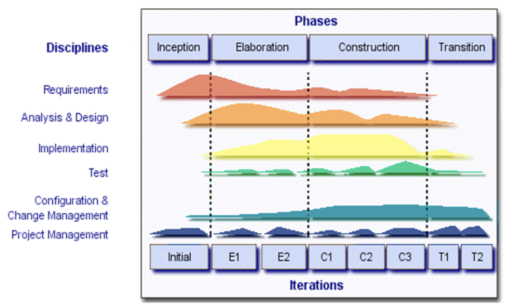
\includegraphics[width=0.48\textheight]{figures/UP-model.png}}
    \caption{UP forløb. \cite{UPModel} } \TODO husk ref
    \end{center}
\end{figure}

%Beskrivelse af vores projektplanlægning
\subsection{Planlagte forløb}
\begin{flushleft}
Vi har efter gode erfaringer i CDIO-2 planlagt, at sætte os ned samlet i gruppen, for at få fastsat datoer for, hvornår hver fase af projektet  ønskes færdigt. Her blev vi enige om at inception-fasen for projektforløbet, skulle være færdigt d. 6. november, hvor kravspecifikationer og vigtigste use-case udarbejdes.\newline

Elaboration-fasen for projektet valgte vi, at have deadline d. 7.november. Denne fase dækker over, at analyse af systemet afsluttes, design påbegyndes og kodeansvar uddelegeres mellem gruppemedlemmer. \newline

Deadline for konstruktionsfasen af projektet blev vi enige om, at opdele i to mindre iterationer. Den første valgte vi at sætte til d. 13. november, som dækker over nogle væsentlige klasser i systemet, der gør det muligt at arbejde videre på \textit{Game}. Den anden del af fasen blev sat til d. 18. november, som primært dækker over \textit{Game} færdiggøres. I begge iterationer for konstruktionsfasen planlagde vi at implementering og test af kode samt opdatering af design artifaktor udarbejdes og bliver færdiggjort. Alt dette skulle derudover løbende dokumenteres i en rapport, hvis deadline blev sat til d. 25. november. Dette projektforløb kan derfor opstilles i et Gantt-kort på følgende måde:
\end{flushleft}

%Gantt-kort for planlagte forløb
\begin{figure}[H]
    \begin{center}
   {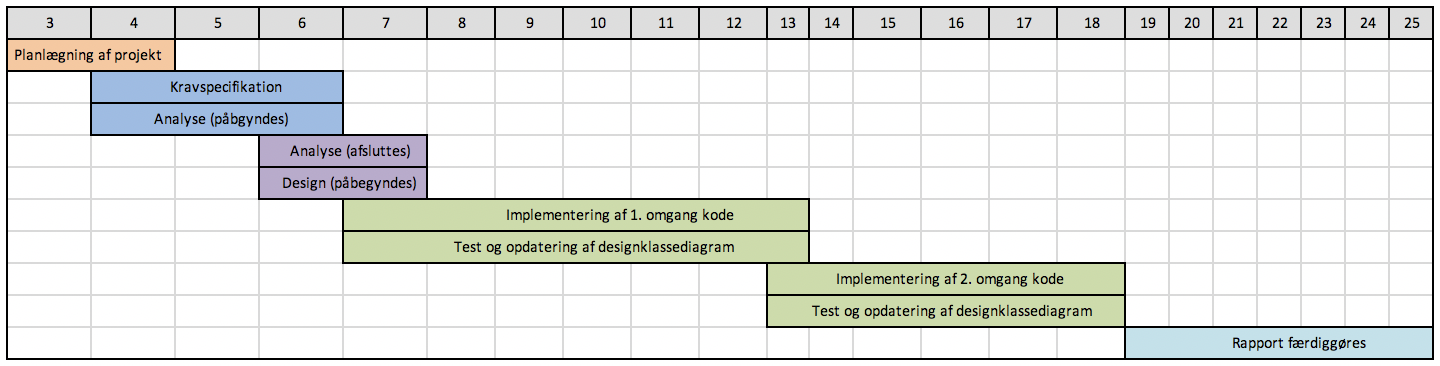
\includegraphics[width=0.7\textheight]{figures/Gantt-1.png}}
    \caption{Gantt-kort for planlagte forløb}
    \end{center}
\end{figure}  


\subsection{Faktiske forløb}

%Gantt-kort for faktiske forløb
\begin{figure}[H]
    \begin{center}
   {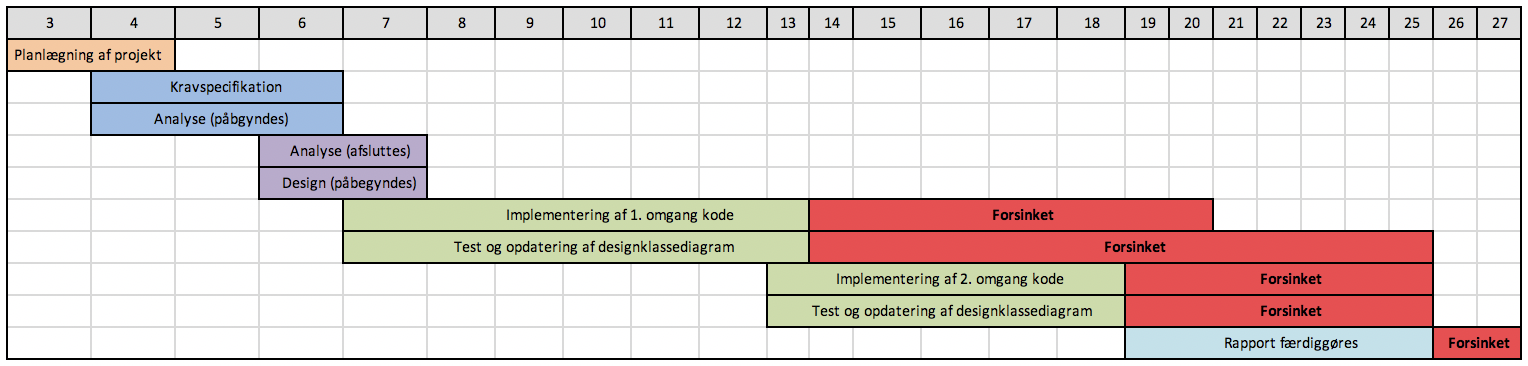
\includegraphics[width=0.7\textheight]{figures/Gantt-2.png}}
    \caption{Gantt-kort for faktiske forløb}
    \end{center}
\end{figure}

\begin{flushleft}
I vores faktiske forløb af projektet, havde vi som sagt valgt at have samme fremgangsmåde, som i vores tidligere CDIO-projekter. Det vil sige at alle har været med inde over arbejdet i inception-fasen. Her er opgavebeskrivelsen blevet læst grundigt igennem, der er opstillet kravspecifikationer og påbegyndt vigtiste analyse-elementer. Dette har bl.a. været med til vi tidligt i processen har kunne definere spørgsmål til kunden, omkring kravspecfikationen og opgavebeskrivelsen. Derudover har det også givet anledning til, at skabe en mere intuitiv overgang til design-fasen af systemet. Årsagen til dette skyldes, at alle har været på lige fod i forbindelse med, hvad der forventes af kunden. Som det kan aflæses på Gantt-kortet har vi ikke haft nogle betydelige forsinkelser ift. det der blev planlagt i denne fase. En vigtig pointe at have med fra denne del af projektet er, at kunden har været længere om, at vende tilbage på enkelte spørgsmål end forventet. Dette har gjort vi først har kunne afslutte dele af kravspecifkationen til sidst i projektforløbet, hvilket normalt ikke er optimalt og kan have store konsekvenser. Dog har disse krav ikke haft den største påvirkning på vores videre arbejde, men kunne have haft væsentlig betydning, hvis der var tale om mere essentielle krav. \newline

I elaboration-fasen blev analysen af projektet færdiggjort og design blev påbegyndt i fælleskab. Ud fra vores udarbejdede designklassediagram valgte vi, at uddelegere kodeansvar blandt gruppemedlemmerne. Dette gjorde vi ved, at opstille diverse klasser i en tabeloversigt og for nogle klasser, også korte underpunkter ift. hvad der skulle udarbejdes. Igen kan det ses på Gantt-kortet at tidsestimeringen af fasen holder stik. \newline

I konstruktion-fasen af forløbet, begyndte der dog at opstå flere komplikationer, end vi havde forventet os. Som nævnt i det planlagte projekt, har vi taget ved lære fra CDIO-2, hvor vi fandt ud af det er en god idé at tage højde for, om der er elementer af kode, der skal være færdiggjort før andet kan påbegyndes. Dette så vi som en rigtig god idé.Vi oplevede dog i første del af konstruktion-fasen, den klart største forsinkelse for projektet. Her blev det planlagt at være færdig med diverse implementeringer d. 13. november, men disse endte først med at være færdige omkring d. 25. november - altså den dag det faktisk var planlagt, at hele projektet ville være færdigt og afleveret til kunden. Denne forsinkelse har derfor også medført at \textit{Game} har måtte blive udskudt. Heldigvis var det planlagt fra vores side af, at deadline ville være tidligere end afleveringsfristen, så vi har haft tid nok til så vidt muligt at rette op på uforudsete problematikker.\\ Hvad har så været skyld i forsinkelserne? Der har været flere årsager til forsinkelse af projektet. Et af de første vi støtte på var, at vi i gruppen valgte at arbejde med elementer, som ikke har været på pensum i undervisningen og ikke alle har haft erfaring omkring før - her er der tale om XML og ArrayList. Denne indragelse har gjort, at vi i gruppen løbende har skulle forsøge, at sætte os ind i hvordan XML-implementeringen fungerer og finde ud af hvordan ArrayList virker. Alt dette skulle gøres parallelt med vi har skulle implementere kode, som forudsætter kendskab til ovenstående, og derudover også samtidigt arbejdet på andre projekter i samme kurser og andre kurser, som vi havde glemt at tage højde for i projektplanlægningen. I forbindelse med ArrayList valgte vi dog senere i projektet, at finde en metode hvorpå Arraylist kunne undgås.\vspace{4mm}
Derudover har en af de helt store faktorer for forsinkelsen også været, at der ikke er blevet lagt nok tid i, at være præcise nok i hvad der faktisk skal laves. Et godt eksempel på dette var, at vi først d. 16. november, blev enige om at definere en Deck-klasse til systemet. Dette burde vi allerede i elaboration-fasen havde tænkt over i design-delen af projektet. Generelt set har der været flere mindre ting, som kunne være undgået, ved et bedre og mere fyldestgørende design. \TODO[\textit{Skal måske omskrives-->}]Set på den positive side, har vi været gode til at opstille møder, når der har opstået problemer. Til disse møder har vi bl.a. talt om, hvad der kan gøres for, at vi kan nå mest muligt af vores projekt - her valgte vi ofte at udskyde deadline, da vi har haft tid nok i sidste ende eller generelt bare rådgivet hinanden undervejs.\vspace{4mm}

Vi har derfor fremadrettet lært, at bruge mere tid i udarbejdelse af design, så disse tanker bliver udtænkt inden de bliver forsøgt kodet. Derudover vil en grundigere udarbejdelse af design klassediagrammet også gøre, at alle i gruppen har en idé om samspillet mellem klasserne og metoderne.\newline

........ Er ikke skrevet helt done endnu, da vi ikke er færdige:)

\end{flushleft}

\end{document}